\documentclass{article}
\usepackage{graphicx} % Required for inserting images
\usepackage{algorithm} 
\usepackage{subcaption}
\usepackage{algpseudocode} 
\usepackage{comment}
\usepackage[
backend=biber,
style=alphabetic,
sorting=ynt
]{biblatex}
\usepackage{hyperref}
%\usepackage{cleverref}
%\usepackage{layouts}
\usepackage{graphicx}

\usepackage{adjustbox}

\usepackage{amssymb}
\usepackage{amsmath}
\usepackage{csquotes}
% \usepackage{subfigure}
\usepackage[english]{babel}
\newtheorem{theorem}{Theorem}
\addbibresource{reference.bib}

\newcommand{\bO}{\mathcal{O}}
% set margins
% \usepackage[bottom=0.5cm, right=1.5cm, left=1.5cm, top=1.5cm]{geometry}
\usepackage[margin = 2.5cm]{geometry}

\title{An Overview of Sketching Techniques Comparison for Randomized Numerical Linear Algebra}
\author{Yuqi Liu, Leon Mikulinsky, Konstantin Zörner}

\date{October 2024}

\newtheorem{corollary}{Corollary}[theorem]
\newtheorem{lemma}[theorem]{Lemma}
\begin{document}

\maketitle

\section{Introduction}
Due to the ubiquity of linear algebra in applied mathematics, dimension reduction and memory saving have been  perpetual topics as there is an ever-increasing demand for solving larger problems faster. However, numerical linear algebra's potential in this field has been well understood and exploited. On the other hand, randomized linear algebra (RLA) is a promising field that still has considerable space for utilization. In 1984, it was discovered that projecting onto a random basis approximately preserves pairwise distances with high probability~\cite{beals1984conference}, thereby opening the doors to using randomized techniques to solve previously difficult or expensive problems.

Sketching -- the process of reducing a standard linear algebra problem to a smaller, more tractable one by projecting the matrix of interest to a lower-dimensional subspace --  forms the backbone of aplty named sketch-and-solve RLA algorithms and is thus essential to building a deeper understanding of the subject. As such, in this paper, we focus on this important building block rather than one individual example of a particular RLA routine. 

A large variety of different techniques has been proposed to construct a random sketching operators. Further, different linear algebra problems lead themselves to different matrix structures, and as such, to different sketching matrix structures. Therefore, this paper focuses on investigating which sketch matrix structures are most suitable for a number of sample problems, both from the theoretical and computational perspective.


%In that regard, we hope to investigate whether some sketching methods favor time of accuracy or vice versa.\cite{9414030} Similarly, we would like to see which techniques for sketching work particularly well with certain linear algebra problems while performing weaker in different settings, and also to investigate how the structure of the original matrix A (e.g. sparsity, or lack thereof) plays a role in a sketch matrix’s effectiveness.\\
%To be more precise, we propose investigating different sketch matrix structures, and see how suitable they are for all kinds of solutions such as least-squares, low rank approximation, and matrix leverage score calculations. We will try to investigate the tradeoffs involved with the following sketch matrix architectures: Gaussian i.i.d. matrices, random sign matrices, Fourier and Hadamard transform-based matrices, along with CountSketch and OSNAP matrices. This wide variety of sketch matrix designs, which include dense, structured, and sparse structures, will allow us to present a bird’s-eye view of the different random NLA techniques currently in use.\\


\section{Literature Review}

Randomized sketch-and-solve algorithms consist of two steps: first, reduce the problem to one of a smaller dimension, and secondly, apply the deterministic algorithm to the reduced problem. This survey focuses on analyzing the first step.

In the following section, we present a number of sketching matrix  $S$ architectures. In this paper, we discuss left-sketching, that is, projecting the target matrix $A$ to $SA$. Unless otherwise noted, the original matrix $A$ is $m \times n$, and the sketching operator $S$ is $k \times m $, where $k \leq m$.

\subsection{Preliminaries}
\label{sec:preliminaries}
Sketching matrices are linear maps defined as $(1\pm \varepsilon) \ell_2$ embeddings 
\begin{equation}
\label{eq:ebedding_property}
    (1 - \varepsilon) \|Ax\|^2_2 \leq \|SAx\|^2_2 \leq (1+\varepsilon) \|Ax\|^2_2
\end{equation}
with a certain probability depending on the structure of $S$, which represents how much $SA$ deviates from being an isometry for $A$. The distortion $\varepsilon$ can be explicitly calculated as follows \cite{magdonismail2019fastfixeddimensionl2subspace}:
\begin{equation}
\label{eq:distortion}
    \varepsilon = \|I - (A^TA)^{-1/2} (SA)^T (SA) (A^TA)^{-1/2}\|_2
\end{equation}

\subsection{Random Orthogonal Matrices}


Arguably, one of the simplest sketch matrix types is the random orthogonal matrix, which is sometimes referred to as Haar operators. It is defined in the Johnson–Lindenstrauss lemma~\cite{https://doi.org/10.1002/rsa.10073,Johnson1984ExtensionsOL}, which states the following:
\begin{lemma}
For $0 < \varepsilon < 1$ and any integer $n$, for $k \geq 8\varepsilon^{-2}\log n $, then for any set $X$ of $n$ vectors in $\mathbb{R}^m$, there is a random orthogonal matrix scaled by $\sqrt{m/k}$, $S$, such that for all $x_i \in X$
\begin{align*}
    (1 - \varepsilon)||x_i - x_j||_2^2 \leq ||S (x_i - x_j)||_2^2 \leq  (1 + \varepsilon)||x_i - x_j||_2^2
\end{align*} 
for all $1 \leq i, j\leq n, i \neq j$ with probability greater than or equal to $1/n$.\end{lemma}


Naively, this allows the construction of a sketching matrix through the following algorithm:
\begin{enumerate}
    \item Generate a random $k \times m$ matrix $M$ whose entries are, say, i.i.d. gaussian, i.e. $(M)_{ij} \sim \mathcal{N}(0, 1)$.
    \item Decompose $M$ to its $QR$ factorization, where $Q$ is orthogonal and $R$ is upper triangular, and store $Q$.
    \item  Set $S = \sqrt{\frac mk} \; Q$.\footnote{This is justified by the fact that sketching matrices $S$ are defined to preserve expectations($\mathbb{E} \|Sx\|_2^2 = \|x\|_2^2$) due to its embedding property \cite{Nakatsukasa2024accuraterandomizedalgorithms}}.
\end{enumerate}

Unfortunately, in order to achieve low distortions, the random orthogonal matrix defined by the Johnson-Lindenstrauss lemma is impractical due to the fact that the embedding dimension is proportional to $\varepsilon^{-2}$, making it difficult to achieve low distortions \cite{martinsson2021randomizednumericallinearalgebra}. Moreover, the sketching process itself may be rather prohbitive because it nessesitates running the $QR$ decomposition algorithm (which takes $\bO(mk^2)$ on a wide left-sketching matrix) as well as multiplying $S$ and $A$ (which takes $\bO(mnk)$ operations).


\subsection{Dense sketching operators}
\label{sec:Dense sketching operators}
In dense sketching operators, we sample sketching operators with i.i.d. entries drawn from particular distributions. We introduce three kinds of operators for this survey, noting that depending on the dimensions of the problem, they may need to be rescaled to preserve isometry: 
\begin{itemize}
   \item \textbf{Rademacher sketching operators}: entries are $\pm 1$ with equal probability.
    \item \textbf{Uniform sketching operators}: entries are sampled from a uniform distribution over a symmetric interval.
    \item \textbf{Gaussian sketching operators}: entries are sampled from a normal distribution with mean $0$.
\end{itemize}

Universality principles in high-dimensional probability \cite{oymak2018universality} guarantee that these sketching operators are practically equivalent \footnote{This applies to any such matrix when each of the entries are independent random variables, have mean $0$ and variance $1$, are drawn from a symmetric distribution, and have uniformly bounded moments \cite{oymak2018universality}.}, which is also highlighted in our results. 

%For the sake of completeness, all three are included in this survey. It should be noted that sketching with Rademacher matrices may be implemented more efficiently than with i.i.d. Gaussian or uniform sketching operators since the matrix multiplication of $SA$ does not require any multiplication in the dot product computation -- only addition and subtraction.%

%These sketching matrices are primarily used for low rank approximation and not the least-squares problem, when the primary purpose of the sketching operator is to sample the matrix in question, rather than to embed it into a smaller subspace, a fact which is proven infeasible due to the generally expensive nature of sketching with them \cite{murray2023randomizednumericallinearalgebra}.


%We will investigate at their implementation efficiency and the intended use cases for these operators. Sampling from the Rademacher or uniform distributions is the most basic operation of random number generators. Methods for sampling from the Gaussian distribution involve transforming random variables sampled uniformly from $[0,1]$~\cite{murray2023randomizednumericallinearalgebra}.

The intended use case for dense sketching operators is mainly sketching in the sampling regime, where the sketching operator is far smaller than the data to be sketched. When the sketching matrix is larger than the data to be sketched, these distributions are much less useful because they are more expensive to apply to dense matrices\cite{murray2023randomizednumericallinearalgebra} -- indeed, although for $S$ a $k \times m$ sketching operator, the distortion for a sketched matrix $\varepsilon \in \Theta(\sqrt{ n/k})$, where $A$ is $m \times n$ \cite{magdonismail2019fastfixeddimensionl2subspace}.


\subsection{Sparse sketching operators}
Sparse sketching operators are often constructed by independently generating the rows or columns of the sketching operator. Nevertheless, it should be noted that there exists another type of sparse sketching operator -- the i.i.d. sparse sketching operator -- constructed by randomly setting many of a dense sketching operator's entries to $0$. However, because of their random structure, their theoretical guarantees are not as robust as the aforementioned row-by-row or column-by-column sketching operator \cite{murray2023randomizednumericallinearalgebra}.

%can be classified as either sort-axis-sparse (SASO) or long-axis-sparse operators (LASO) \cite{murray2023randomizednumericallinearalgebra}, where the short and long axes correspond to the rows and columns (resp. columns and rows) of a wide (resp. tall) matrix. These correspond to how the sketch matrix is constructed: whether its "long" or "short" axis elements are independent from one another. As such, a SASO matrix has independent short axis vectors (e.g. columns in a wide matrix or rows in a tall matrix), with the opposite applying to LASOs.

%Because this work focuses exclusively on left-sketching (i.e. sketching of the form $SA$ as opposed to $AS$),%
%In our work, we will primarily discuss SASOes. %which are more commonly used for this sketching method. 
%It should be noted that there exists another type of sparse sketching operator which is the i.i.d. sparse sketching operator, constructed by randomly setting many of a dense sketching operator's entries to $0$. However, because of their random structure, their theoretical guarantees are not as robust as the aforementioned operators \cite{murray2023randomizednumericallinearalgebra}.

A prototypical example of a sparse sketching operator is the Clarkson-Woodruff transform (CWT), also known as the CountSketch matrix \cite{10.1145/3019134}. This matrix is generated by choosing one element in each of its columns to be equal to $\pm 1$ with equal probability, and setting the rest to $0$. Using this as a sketching matrix, we have that the distortion $\varepsilon \in \Theta(\sqrt{n^2/k})$ \cite{magdonismail2019fastfixeddimensionl2subspace}.

This can be generalized to a Sparse Sign Embedding (SSE) \cite{9414030}, which can contain more than one non-zero entry per column. Namely, for a $k \times m$ SSE matrix $S$ and parameter $p\in(0, 1)$, it satisfies 

\begin{equation}
    S = \alpha s_{ij}, \qquad s_{ij} \sim \begin{cases}
        +1 \text{ with probability } p/2 \\
        -1 \text{ with probability } p/2 \\
        0 \quad\text{otherwise}
    \end{cases} 
\end{equation}

where $\alpha =  \frac{1}{kp}$ is a normalizing factor included to ensure $S$ has an expectation of $I_m$ \cite{tropp_2023_0na16-j0x38}.

%Sparse sign matrices satisfy the following bound:\\

\textit{For $S$ $k\times m$, $p \in (0, 1)$, $C_1, C_2$ positive constants and the following condition:  
\begin{equation}
    k \gtrapprox  C_1 (d + \log m) \log d, \qquad  p \gtrapprox C_2 \frac{\log d}{k}
\end{equation}
then with high probability, for any $d$-dimensional subspace, $S$ is an embedding with constant distortion $\frac{1}{2}$} \cite{tropp_2023_0na16-j0x38}.

These can also be generated by specifying a sparsity parameter $\zeta$ to represent the number of non-zero elements per column. Analogously, it has been shown that a sparse sign matrix serves as a subspace embedding with high probability with constant distortion for an arbitrary $l$-dimensional subspace of $\mathbb{R}^m$ when the embedding dimension grows $\bO(d \log d)$ and the sparsity parameter $\zeta$ as $\bO(\log d)$ \cite{martinsson2021randomizednumericallinearalgebra}.

\subsection{Subsampled Random Trigonometric Transformations}
Fast trigonometric transforms are orthogonal or unitary operators that take m-vectors to m-vectors in $\bO(m \log m)$ time or better. % The most important examples in this class are the Discrete Fourier Transform(for complex valued inputs) and the Discrete Cosine Transform (for real-valued inputs). At the same time, the Walsh-Hadamard Transform is also notable. 
In randomized algorithms, we treasure their ability to map inputs that lack periodic structure to dense outputs, and they are referred to as \textit{subsampled randomized fast trig transforms}.  

These sketching operators are defined as follows \cite{halko2010findingstructurerandomnessprobabilistic}:
\begin{align*}
    S = \sqrt{\frac mk}RTD
\end{align*}

Where $D$ is a $m \times m$ diagonal matrix whose diagonal entries are uniformly distributed around the unit circle in the complex case (and in the real case, $\pm 1$), $T$ is a trigonometric transform, and $R \in \mathbb{R}^{k \times m}$ is a sampling matrix, selecting $k$ rows from the $m \times m$ matrix it multiplies.

Depending on the initial data or other problem parameters, $T$ can be a discrete Fourier transform such that $(T)_{jk} = m^{-\frac12}e^{-\frac{2\pi i}{m}(j-1)(k-1)}$ for $j, k = 1, 2, \dots, m$, the similarly defined discrete sine or cosine transforms, or the discrete Hadamard transform, where $T = H_m$ for $m = 2^n$ and:\\
\begin{align*}
    H_m = \begin{bmatrix} H_{m/2} & H_{m/2} \\ H_{m/2} & -H_{m/2} \end{bmatrix}, \qquad H_2 =  \begin{bmatrix} 1 & 1 \\ 1 & -1 \end{bmatrix}
\end{align*}

Thus, the Hadamard transform functions as a sort of analoughe for the Fourier transform for real data, having a distortion $\varepsilon \in \Theta(\sqrt{(n \log n)/d})$ \cite{magdonismail2019fastfixeddimensionl2subspace}. It should be noted that although $S$ can be represented as a nested series of matrix multiplications, in practice, the sketching operator can be applied to each column vector $x$ of the initial matrix $A$ by scaling (multiplication by $D$, applying the trigonometric transform like the DFT (multiplication by $T$), and then randomly sampling the result (multiplication by $R$), thereby reducing the sketching operation to be of order at most $\bO(mk\log m)$ for each column vector. For all practical applications, this is how the algorithm is implemented.\\


\textit{For a positive constant $C$ and for $k \gtrapprox C (d + \log m) \log d$, then with high probability, for an $d$-dimensional subspace, the SRFT matrix $S$ is a subspace embedding with distortion $\frac12$}\cite{tropp_2023_0na16-j0x38}.\\

Curiously, although theoretically SRTTs need the embedding dimension to grow as $\bO (d \log d)$ as above, it is often sufficient to to choose an embedding dimension of only $\bO(d)$ \cite{martinsson2021randomizednumericallinearalgebra}.
%SRFTs are appealing for their efficiency and theoretical guarantees\cite{WOOLFE2008335}. However, it is pointed out in some paper~\cite{murray2023randomizednumericallinearalgebra} that block SRFTs~\cite{balabanov2022blocksubsampledrandomizedhadamard} are worth more attention than the traditional one. 
%In the book, they use a taxonomy for sparse sketching operators which has not appeared in prior literature: To describe it, we use the term short-axis vector in reference to the columns of a wide matrix or rows of a tall matrix. The term long-axis vector..

\subsection{Properties of Sketching Matrices and Sketch Quality}

Now that we have introduced all of the sketching methods that we will use we can look back at the two properties \hyperref[eq:ebedding_property]{(\ref*{eq:ebedding_property})} and \hyperref[eq:distortion]{(\ref*{eq:distortion})} introduced in \hyperref[sec:preliminaries]{Section~\ref*{sec:preliminaries}}. In practice, it oftentimes suffices to require a relaxed version of property \hyperref[eq:ebedding_property]{(\ref*{eq:ebedding_property})}, namely it suffices if a sketching matrix preserves relative norms \cite{murray2023randomizednumericallinearalgebra}, i.e. 
\begin{equation}
    \frac{\Vert Su\Vert_2}{\Vert Su\Vert_2} \approx \frac{\Vert u\Vert_2}{\Vert v \Vert_2}
    \quad \text{for } u, v \in \mathrm{col}\{A\}.
\end{equation}

To illustrate that the introduced sketching methods fulfill this property we depict how they impact the relative norm in \hyperref[fig:sketch_properties]{Figure~\ref*{fig:sketch_properties}} along side the computed distortion of some of the sketching methods for a matrix $A \in \mathbb{R}^{1024 \times 50}$ with entries i.i.d. sampled form a standard normal distribution.



\begin{figure}[htb]
  \centering
  \begin{minipage}[t]{.49\linewidth}
    \centering
    \adjustbox{valign=t}{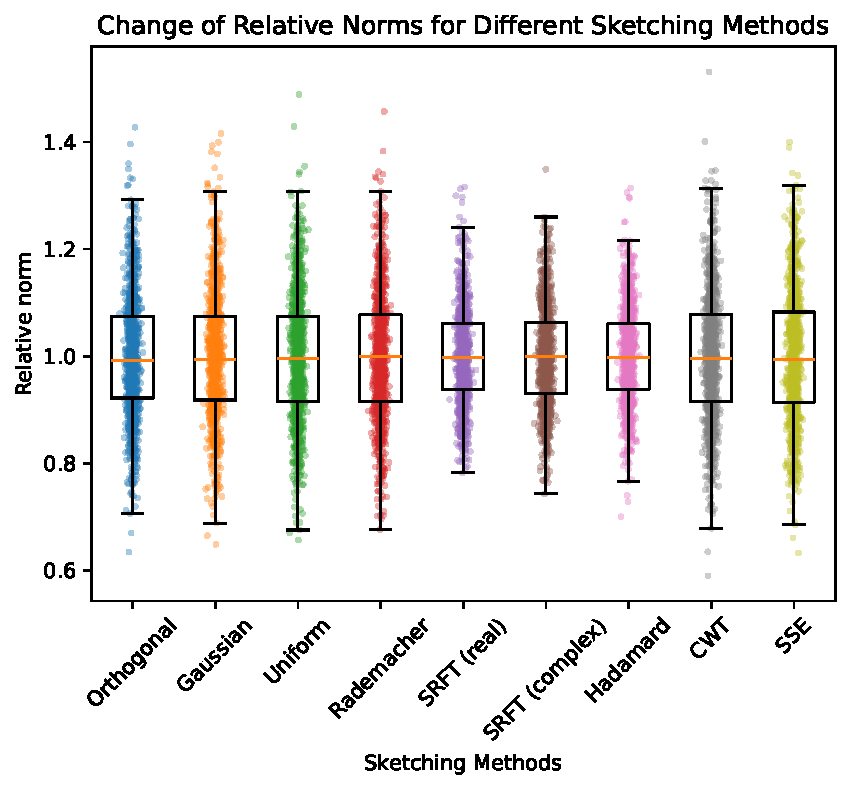
\includegraphics[width=\textwidth]{figures/sketching_properties/relative_spread_box_plot34069384.pdf}}
  \end{minipage}
  \begin{minipage}[t]{.49\linewidth}
    \centering
    \adjustbox{valign=t}{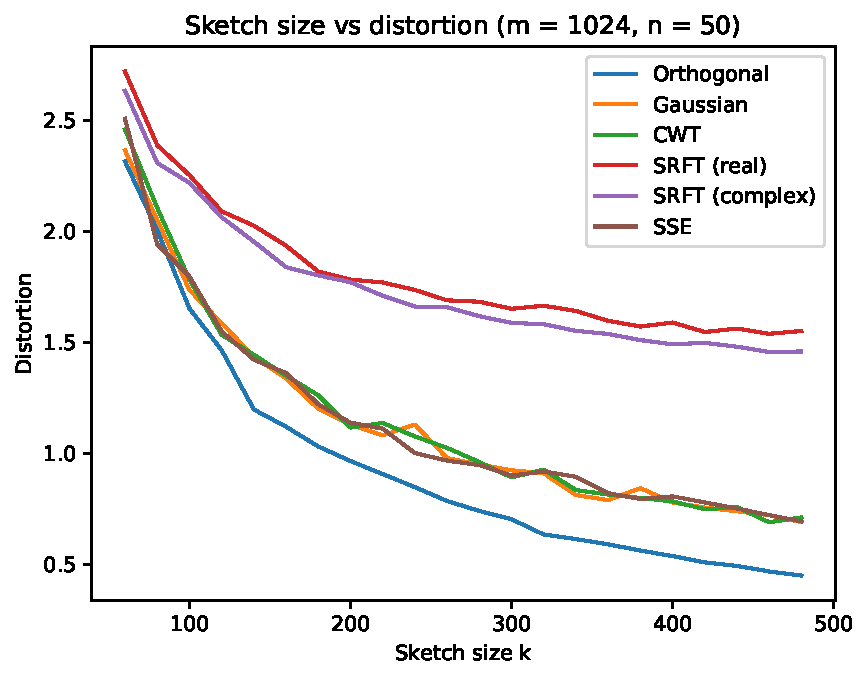
\includegraphics[width=\textwidth]{figures/sketching_properties/sketch_size_vs_distortion34066431.pdf}}
  \end{minipage}
  \caption{Illustration of the embedding property for different sketching methods (left). Distortion for a matrix $A \in \mathbb{R}^{1024 \times 50}$ with i.i.d. standard normal entries for different sketching methods (right).}
  \label{fig:sketch_properties}
\end{figure}


\section{Test Problems}
\subsection{Low-Rank Approximation}
The low-rank approximation problem could be stated as follows:\\

\textit{Given an $m \times n$ matrix $A$, find a matrix $A_k$ such that} \text{rank}$(A_k) = k \ll \min(m, n)$ \textit{and $\| A - A_k\|$ is minimized.}\\

There are two primary approaches to solving this problem that are best exemplified through the following algorithms:
\begin{itemize}
    \item \textbf{Singular Value Decomposition}: Factorizing the target matrix as $A = U \Sigma V^T$ with $U, V$ orthogonal and $\Sigma$ diagonal. By denoting $u_i$ and $v_i$ to be the column vectors of $U$ and $V$ respectively and $\Sigma = \text{diag}(\sigma_1, \dots, \sigma_n)$ and using the convention that $\sigma_1 \geq \dots\geq\sigma_n=0$, we can also write $A$ as follows $ A = \sum_{i=1}^n \sigma_i u_iv^T_i$ and form $A_k$ by truncating the sum at some $k \leq n$. This approach, which gives the best possible rank $k$ approximation by the Eckart-Young-Mirsky theorem, is often computationally infeasible.  Similar algorithms can be used if $A$ has a special structure, such as symmetry.
    \item \textbf{$CUR$ decomposition}: For $A$ an $m \times n$ matrix, the $CUR$ decompositon is formed by selecting small subsets of $A$'s columns in the $m \times k$ matrix $C$, rows in $k \times n$ matrix $R$, and linking the two using $k\times k$ matrix $U$ such that $A_k = CUR$. Serving as a representative of submatrix-oriented decompositions, these algorithms, though more prone to numerical instability, can require less storage to compute than SVD-like decompositions, especially when $A$ is sparse. 
\end{itemize}

Nevertheless, using randomized techniques on the low-rank approximation problem can lead to improved efficiency and stability, if the right sketching operator is chosen, especially for large matrices target matrices where these algorithms would prove otherwise infeasible (e.g. the SVD decomposition taking $\bO(mn^2)$).

%\begin{itemize}
%\item[$\bullet$]Spectral decomposition:this consists of low-rank SVD and Hermitian eigendecomposition.
%\item[$\bullet$]Submatrix-oriented decomposition:CUR decomposition and interpolative decompositions.
%\end{itemize}
%To solve low-rank approximation from sketching matrices, we have a lot of drivers to follow. To discuss these drivers for low-rank approximation, it is necessary to mention briefly the following two concepts.

%\begin{itemize}
%\item[$\bullet$]A QB decomposition is a simple representation that is useful for SVD and eigendecomposition. The representation taks the form $\hat{A}=QB$ for a tall matrix with orthonormal columns and $B=Q^*A$. The important point here is that the QB decomposition involves explicit construction of and access to both Q and B.
%\item[$\bullet$]
%Column subset selection(CSS) is the problem of selecting from a matrix a set of columns that is "good" in some sense. CSS algorithms largely characterize algorithms for one-sided ID. They are important here because a one-sided ID can be used for the simple representation of $\hat{A}$ when working toward an SVD, eigendecomposition, two-sided ID, or CUR decomposition. 
%\end{itemize}
%Low-rank approximation has been important in reducing the size of data while randomized algorithms definitely help to reduce the computation it needs.

%Here we mainly use randomized SVD as our example of illustration; the steps of randomized SVD could be divided into two parts.  

%To test the efficiency and accuracy of sketching matrices, we chose randomized SVD with different sketching matrices to test how it compares to standard SVD when we get the same-rank approximation. The randomized SVD algorithm could be partitioned into two parts; first, we use randomization to compute a QB decomposition of the input matrix A, and then we deterministically compute QB's compact SVD, and finally, truncate that SVD to a specific rank.

%To do Hermitian decomposition, each randomized algorithm for low-rank SVD has a corresponding version that is specialized to Hermitian matrices. We recount those specialized algorithms here.But there is still an algorithm that is unique to the approximation of psd matrices.

%In general , we shall say that $A$ is $n\times n$ and the algorithms represent $\hat{A}=V diag(\lambda) V^*$, where $V$ is a tall column-orthonormal matrix and $\lambda$ is a vector with entries sorted in decreasing order of absolute value.


Before we start our low-rank approximation, we first introduce one of the building blocks for low-rank approximations, which is called QB decomposition; here we borrow the practice taken in \cite{yu2018efficientrandomizedalgorithmsfixedprecision} as a representative. See algorithm \ref{algorithm 1} as a reference. And the
\begin{algorithm}
	\caption{The basic QB algorithm to solve rangefinder problem} 
    \textbf{Input}:A,k,s\\
    \textbf{Output}:Q,B
	\begin{algorithmic}[1]
		\State$\Omega=randn(n,k+s)$
        \State$Q=orth(A\Omega)$
        \State$B=Q^TA$
	\end{algorithmic} 
    \label{algorithm 1}
\end{algorithm}

\begin{algorithm}
	\caption{Randomized singular value decomposition(RSVD)} 
    \textbf{Input}:A,k,s\\
    \textbf{Output}:Q,B
	\begin{algorithmic}[1]
		\State$\Omega=randn(n,k+s)$
        \State$Q=orth(A\Omega)$
        \State$B=Q^TA$
	\end{algorithmic} 
    \label{algorithm 1}
\end{algorithm}
After QB, we could do all sorts of deterministic factorization low-rank approximation algorithms on matrix B~\cite{halko2010findingstructurerandomnessprobabilistic}.%%%

Other than sketching matrices, there are many other questions that need to be considered.
\begin{itemize}
    \item How do we choose the subspace dimension for the random matrix?
     The theory\cite{halko2011finding} indicates that we can select the subspace dimension l to be just slightly larger than the rank r of the matrix ,say, $l=r+p$ where $p=5$ or $p=10$, where the value p is called the oversampling parameter.
    \item Matrix multiplication 
    Matrix multiplication is a highly optimized primitive on most computer systems.
    \item Powering Powering iteration could help matrices without a rapidly decaying spectrum. The powering process goes as follows. Let $B\in F^{m\times n}$ be a fixed input matrix, and let $q$ be a natural number. Let $\Omega\in F^{m\times l}$ be a random test matrix. we form the sample matrix \[Y=(BB^*)^q\Omega\] by repeated multiplication.
    \item orthongonalization The columns of the matrix Y tend to be strongly aligned, so it is important to use a numerically stable orthogonalization procedure such as Householder reflectors, double Gram-Schmidt, rank-revealing QR or TSQR algorithm~\cite{DBLP:journals/corr/abs-0806-2159}.


\end{itemize}


\subsection{Overdetermined Least Squares}
\label{sec:least_squares}
The overdetermined least squares problem is defined as follows: \\

\textit{For $A \in \mathbb{R}^{m \times n}, x \in \mathbb{R}^{n}, b \in \mathbb{R}^{m}$ such that $m > n$, minimize $\|Ax - b\|_2^2$.}\\

This can be solved by a number of deterministic algorithms with various trade-offs between speed, accuracy, and stability, including:
\begin{itemize}
    \item \textbf{Normal equations}:   
        Conceptually the simplest, it solves the problem by letting $x = (A^TA)^{-1}A^Tb$. Despite requiring the least amount of floating point operations of all the following methods, this method method is not very suitable for practical applications because it is unstable for poorly-conditioned $A$.
    \item \textbf{$QR$ decomposition}:
        This method performs the following factorization: $A = QR, Q \in \mathbb{R}^{m \times n}, R \in \mathbb{R}^{n \times n}$ such that $Q$ is orthogonal and $R$ is upper triangular for the solution $x = R^{-1}Q^T$. $QR$ factorization can be achieved through a number of algorithms such as Gram-Schmidt or modified Gram-Schmidt, or those which incrementally construct the result using Householder reflections or Givens rotations. In practice, while all of these algorithms have complexity $\bO(mn^2)$, Householder rotations need the least flops among all four, while still being stable and preserving the orthogonality of $Q$'s columns.
    \item \textbf{Singular Value Decomposition}:
        This method performs the following factorization $A = U \Sigma V^T$, where $U, V$ are orthogonal and $\Sigma$ is diagonal. The SVD van be used to solve the problem by setting $x = V \Sigma^+U^Tb$ where $\Sigma^+$ is the psuedoinverse of $\Sigma$. While the most numerically stable, the SVD takes $\bO(mn^2)$, not to mention the matrix multiplication required to form $x$.
\end{itemize}
However, for $m$ large, the latter two algorithms may become impractically slow.

\section{Experiments}
\subsection{Datasets}
\label{sec:datasets}
For our experiments we use both real life data and synthetic data. 
We use the dataset from MedMNIST\cite{medmnistv1,medmnistv2}. In our experiments, we use the dataset of breast, which consists of three parts: training dataset, validation dataset, and test dataset. We just use the training dataset here which has $546$ data points, see \href{https://zenodo.org/records/10519652} {https://zenodo.org/records/10519652}. 
Another thing that is worth attention is that the data is almost full-rank. It is also worth attention that most of the data points are very ill-conditioned. 
Here we examine some basic statistical descriptions about condition numbers. See Figure \ref{tab:condition} as a reference. 
In addition to that, we use scikit-learn's dataset on Californian housing\footnote{\href{https://scikit-learn.org/1.5/modules/generated/sklearn.datasets.fetch_california_housing.html}{\texttt{https://scikit-learn.org/1.5/modules/generated/sklearn.datasets.fetch\_california\_housing.html}}}
, which is suitable for least squares.
As the dataset contains $20640$ data points we sample a smaller, easier to handle number of $1024$ data points.
Our synthetically generated data are split into three different categories. First, we use matrices A with all entries sampled i.i.d. from a standard normal distribution, these behave very numerically very nicely and serve as a good basecase. Second we use matrices with a singular values that span a wide range, causing a very high condition number. In particular, we select $A = U \Sigma V^T$ with $U, V$ orthogonal and $\Sigma$ diagonal with $\sigma_{ii} = e^{k_i}$, where $k_i$ are equidistantly spread in $\{-10, 10\}$. Last, we utilize multicolinear matrices that we generate by sampling a vector $a$ from a i.i.d. standard normal distribution and then setting $A$'s $i$'th column to $a_i = a + 10^{-6}\theta_i$ where $\theta_i$ are also standard normal random vectors with independent components. 



    
\begin{comment}
    \begin{table}
    \centering
    \begin{tabular}{cc}
      variable   &value \\
      \hline
      mean   &214174 \\
      \hline
       median  & 7550\\
       \hline
       std  & 2092978\\
       \hline
        var &4380555*1e6 \\
        \hline
        min & 647.31\\
        \hline
       max  & 37453104\\
       \hline
       25\%  &3532.6 \\
       \hline
        50\% & 7550.5 \\
        \hline
       75\%  &19286.7 \\
    \end{tabular}
    \caption{Caption}
    \label{tab:condition}
\end{table}
\end{comment}  

 %, which, according to theorem 1 stated in Yu's work as well~\cite{yu2018efficientrandomizedalgorithmsfixedprecision}, that 
%\begin{theorem}
%Let A be an $m\times n$ matrix. Q denotes an $m\times k$ orthonormal matrix($k\textless m$), and $B=Q^TA$. Then,\[||A-QB||_F^2=||A||_F^2-||B||_F^2\]
%\end{theorem}
\subsection{Results}
\label{sec:results}
\subsubsection{Low Rank Approximation}
\label{sec:results_low_rank_apprximation}
Our results are shown in Figure \ref{fig:results on breastmnist boxplot}, and the table containing concrete numbers is shown in 
\begin{figure}[h]
\begin{subfigure}
    {0.5\textwidth}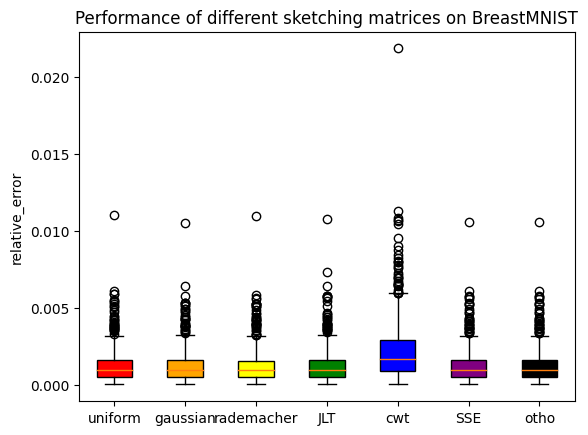
\includegraphics[width=0.9\linewidth,height=6cm]{figures/boxplot_BREASTMNIST.png}
    \caption{Randomized SVD results on BreastMMNIST DATASET}
    \label{fig:results on breastmnist boxplot}
    \end{subfigure}
    \begin{subfigure}
    {0.5\textwidth}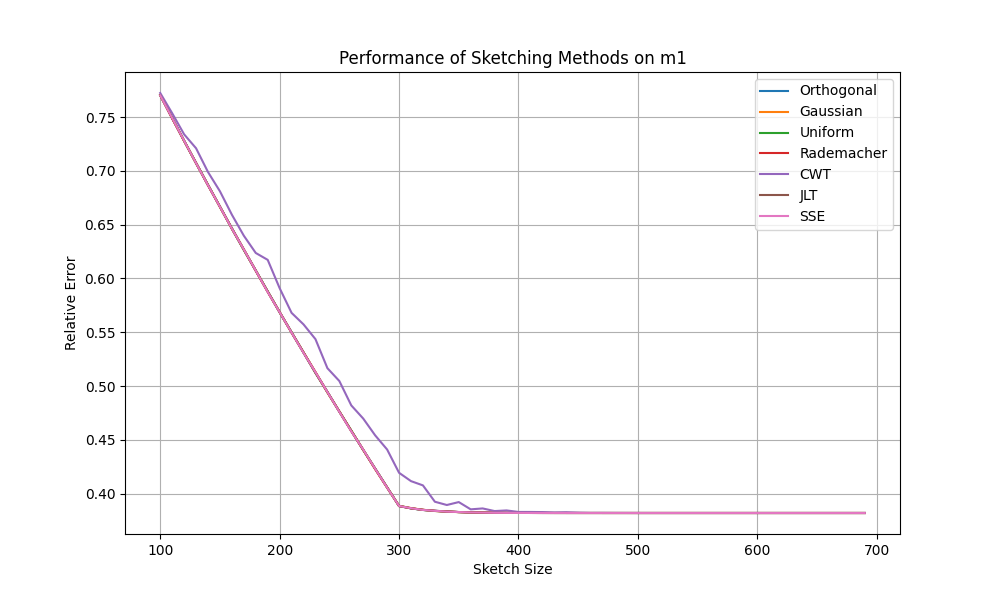
\includegraphics[width=1.0\linewidth,height=7cm]{splines for breastmnist.png}
    \caption{splines for numerical experiments}
    \label{fig:m1_lowrank}
\end{subfigure}
\end{figure}
\ref{tab:table for descriptions}. We also conducted numerical experiments solving the low-rank approximation problem.The result is shown in \ref{fig:m1_lowrank}

\begin{table}
    \centering
    \begin{tabular}{cccccc}
      Sketching Operators   &Uniform  &Gaussian  &Rademacher  & JLT & CWT\\
      \hline
       Mean  &0.001267  & \textbf{0.001257} & 0.001265 & 0.001274 &0.002295 \\
       \hline
       std  & 0.001146 & \textbf{0.001111} & 0.001123 & 0.001154 &0.002231 \\
       \hline
        min & 0.000020 & 0.000019 & 0.000019 & 0.000019 &0.000019 \\
        \hline
        25\% & 0.0000513 & 0.000524 & 0.000532 & 0.000513 & 0.000874\\
        \hline
        50\% &0.000974  & 0.000972 & 0.000971 & 0.000980 & 0.0001709\\
        \hline
        75\% &0.001594 & 0.001600 & 0.001633 & 0.001619 & 0.002860\\
        \hline
        max & 0.011209 & 0.011091 & 0.010804 & 0.010772 &0.015175 \\
    \end{tabular}
    \caption{The Performance of Different Sketching Matrices on breastMNIST}
    \label{tab:table for descriptions}
\end{table}
\subsubsection{Least Squares}
We solved the least squares problem $\min_x \Vert Ax - b \Vert_2$ for the three types of matrices described in \hyperref[sec:datasets]{Section~\ref*{sec:datasets}} using all sketching methods introduced so far using both the QR and the SVD algortithm as outlined in \hyperref[sec:least_squares]{Section~\ref*{sec:least_squares}}. For all choices of $A$ we chose $b$ as a standard normal random vector with independent components. We found both methods to yield the same accuracy so we only depict the results for QR here. 
In order to measure the accuracy of our the different sketching methods we used the following two metrics. First, the relative norm of the residual, i.e.,
$$
\frac{\Vert Ax_{\mathrm{opt}} - b \Vert_2 - \Vert Ax_{\mathrm{sketch}} - b \Vert_2}{\Vert Ax_{\mathrm{opt}} - b \Vert_2},
$$
and second, the relative error of the found $x_{\mathrm{sketch}}$, i.e.,
$$
\frac{\Vert x_{\mathrm{opt}} - x_{\mathrm{sketch}}\Vert_2} {\Vert x_{\mathrm{opt}} \Vert_2}.
$$
repeating these experiments for many different sizes of $A$ yields genuinely similar behavior. Thus, in \hyperref[fig:qr_results]{Figure \ref*{fig:qr_results}} we only chose to depict the results for $A \in \mathbb{R}^{256 \times 20}$. 
\begin{figure}[htb]
  \centering
  \begin{minipage}[t]{.32\linewidth}
    \centering
    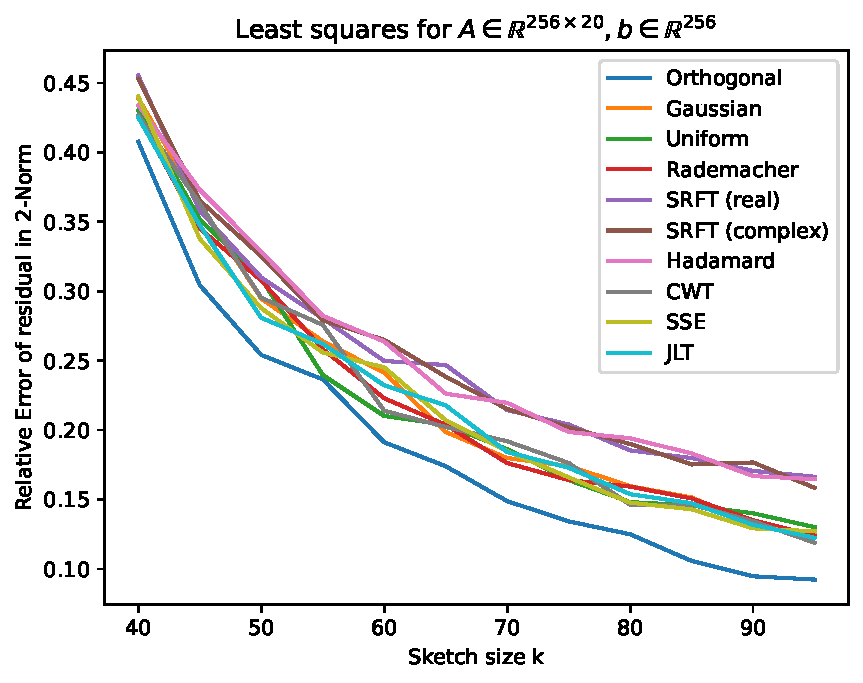
\includegraphics[width=\textwidth]{figures/least_squares/qr_err_vs_k_gaussian_loops100_m256_n2034399542.pdf}
  \end{minipage}
  \begin{minipage}[t]{.32\linewidth}
    \centering
    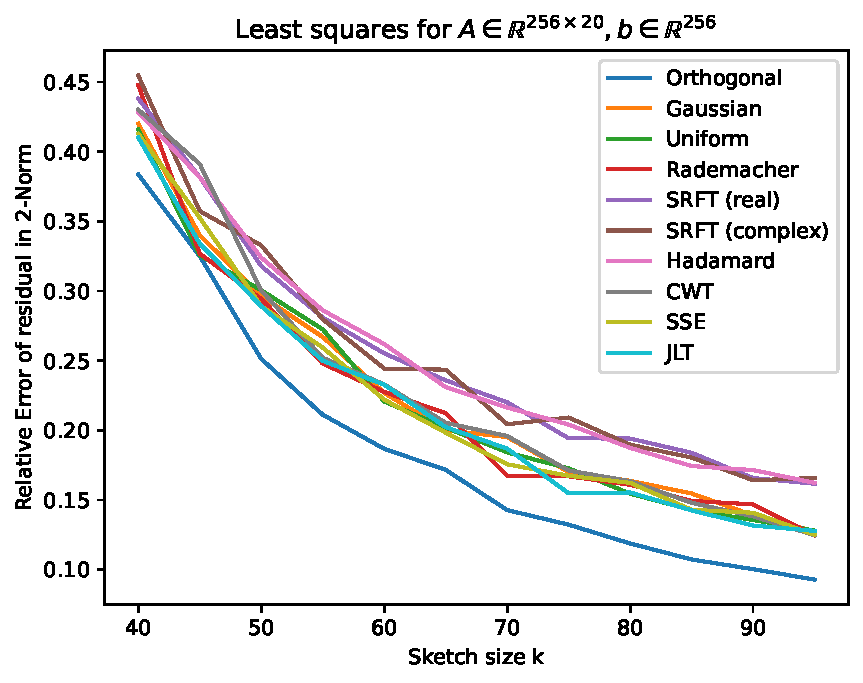
\includegraphics[width=\textwidth]{figures/least_squares/qr_err_vs_k_multicollinerarity_loops100_m256_n2034399459.pdf}
  \end{minipage}
  \begin{minipage}[t]{.32\linewidth}
    \centering
    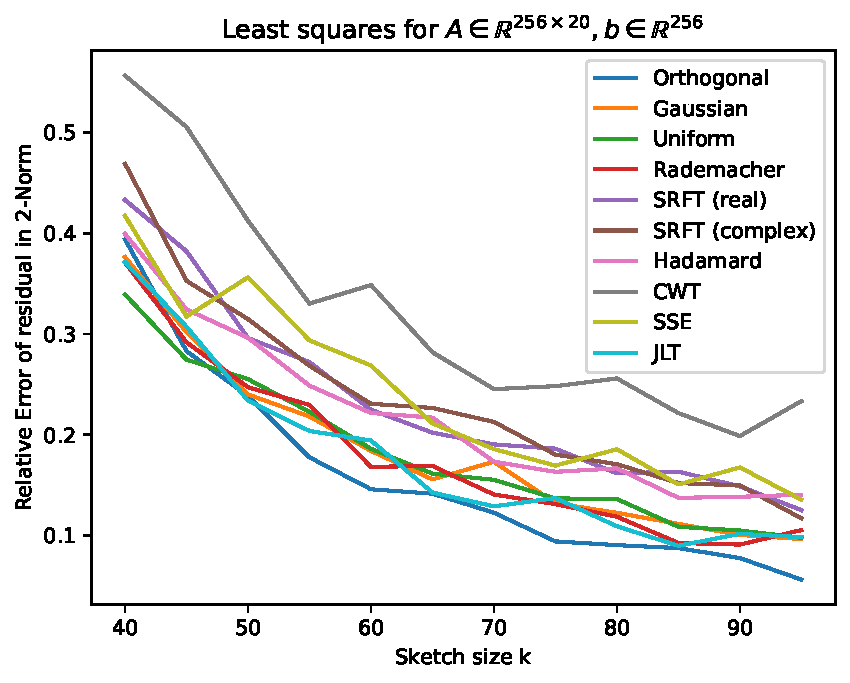
\includegraphics[width=\textwidth]{figures/least_squares/qr_err_vs_k_singular_spread_loops100_m256_n2034399665.pdf}
  \end{minipage}
  \begin{minipage}[t]{.32\linewidth}
    \centering
    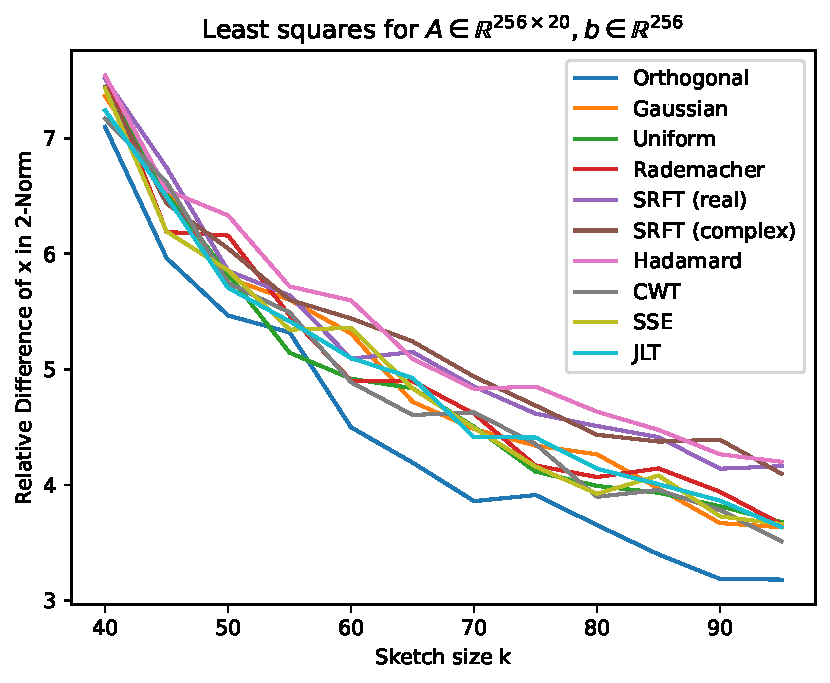
\includegraphics[width=\textwidth]{figures/least_squares/qr_err_vs_k_gaussian_loops100_m256_n2034400377.pdf}
  \end{minipage}
  \begin{minipage}[t]{.32\linewidth}
    \centering
    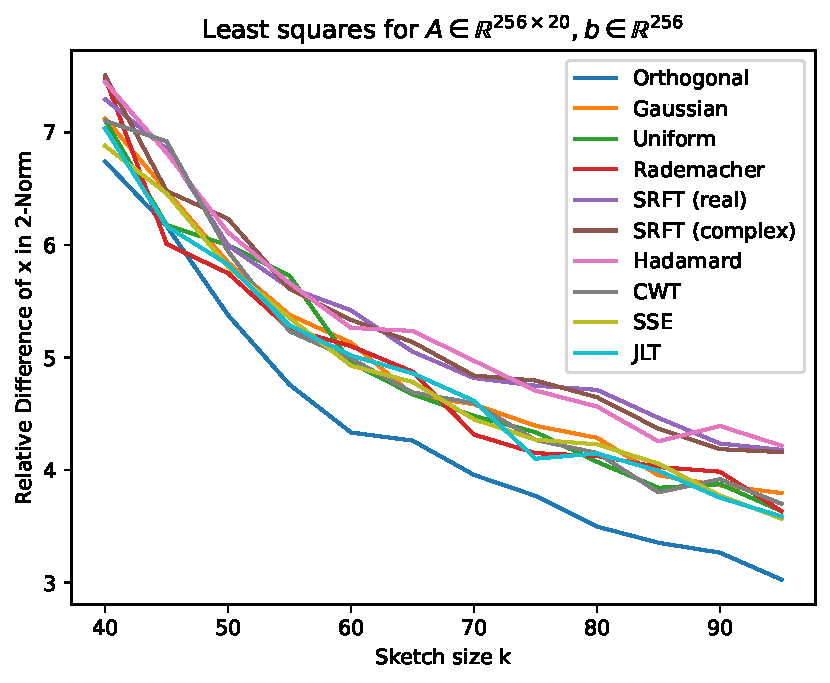
\includegraphics[width=\textwidth]{figures/least_squares/qr_err_vs_k_multicollinerarity_loops100_m256_n2034400280.pdf}
  \end{minipage}
  \begin{minipage}[t]{.32\linewidth}
    \centering
    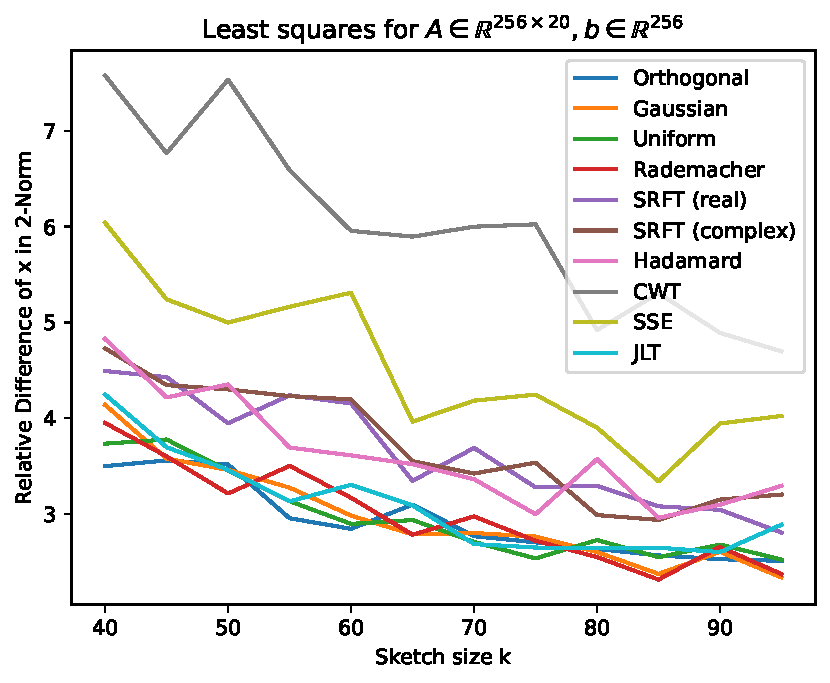
\includegraphics[width=\textwidth]{figures/least_squares/qr_err_vs_k_singular_spread_loops100_m256_n2034400517.pdf}
  \end{minipage}
  \caption{Accuracy of least squares using different sketching methods and different matrices $A$ for i.i.d. Gaussian $b$ averaged over 100 runs each. From left to right $A$ is chosen to be i.i.d. Gaussian, be multicolinear, and have a spectrum spreading 20 orders of magnitude. The relative error of of the residual is depicted at the top and the relative error in $x$ at the bottom.}
  \label{fig:qr_results}
\end{figure}

We repeated the same process for the Californian housing dataset introduced in \hyperref[sec:datasets]{Section~\ref*{sec:datasets}}. Here we found the same behavior for the orthogonal and dense sketching methods. Although and SEE still return good results we observe that CWT's accuracy has significantly gone down, similar to the observations we made for low-rank approximation in \hyperref[sec:results_low_rank_apprximation]{Section \ref*{sec:results_low_rank_apprximation}}. Furthermore, we found that all trigonometric transforms performed much worse on this data set, achieving relative errors for the residual of around 2 across all tested sketching sizes.  



\section{discussion}
Our gathered data presented in \hyperref[sec:results]{Section~\ref*{sec:results}} enables us to make the following observations and allows us to draw some interesting conclusions.
For one we were able to empirically show that all dense i.i.d. sketching operators behave equivalently as proposed in \hyperref[sec:Dense sketching operators]{Section~\ref*{sec:Dense sketching operators}}. This can be clearly seen in \hyperref[fig:low_rank_results]{Figure \ref*{fig:low_rank_results}} where they all cluster achieving similar accuracies regardless of the sketching size $k$. Similarly, the figure suggests that the same might be true for the subsampled random trigonometric transformations, which cluster in a similar manner. 

Next, we conclude, that distortion presents a good measure to indicate the quality of a sketching method (at least for least squares). This can be seen as the clusters found in the distortion plot of \hyperref[fig:sketch_properties]{Figure \ref*{fig:sketch_properties}}) are identical to those found in \hyperref[fig:qr_results]{Figure \ref*{fig:qr_results}}. 

Interestingly, we find that the sparse operators do not form as distinct clusters as the before mentioned groups. For the numerically well behaved Matrix $A$ with i.i.d. standard normal entries we see that they perform just as well as the dense operators. In this case they certainly favorable as their computational cost is $O(nnz)$ compared to the $O(n^3)$ of the dense operators. We observe the same for the multicolinear matrices, however, when it comes to the 
\begin{itemize}

    \item  Distortion is a good measure to indicate the quality of a sketching method (at least for least squares). This can be seen as the clusters found in the distortion plot of \hyperref[fig:sketch_properties]{Figure \ref*{fig:sketch_properties}}) are identical to those found in \hyperref[fig:qr_results]{Figure \ref*{fig:qr_results}}.
    \item For all different types of matrices used to test least squares, we found the same clusters of accuracies. 1. Orthogonal, 2. Dense \& Sparse, 3. SRFTs. Since sparse and dense operators yield similar results, sparse operators are clearly favorable.
    \item For numerically nice matrices $A$ sparse and dense sketching matrices behave alike, clearly favoring sparse matrices. However, for more complicated matrices such as in the third column of \hyperref[fig:qr_results]{Figure \ref*{fig:qr_results}}, sparse sketching matrices struggle to capture $A$ accurately, especially when the number of non-zero entries is low as for WCT. 
    \item jlt outperformce the other sparse operators and still works well for badly conditioned $A$ See  and \hyperref[fig:qr_results]{Figure \ref*{fig:qr_results}}
    \item for given dataset for low rank approximation, k = 300 seems to be sweet spot? (Check whether we can find theoretical guarantees that this is just the right size for k)
    \item TODO: Change low rank approximation results plot to have a logarithmic y-axis
    
\end{itemize}
\printbibliography
\end{document}
